\documentclass[hyperref=unicode]{beamer}
\usepackage[T1,T2A]{fontenc}
\usepackage[utf8]{inputenc}
\usepackage[bulgarian]{babel}
\usepackage{amssymb,amsmath,amsthm,tabu}
\usepackage{tikz}
\usepackage{algorithm,algpseudocode}
\usepackage{graphicx}
\usepackage{tcolorbox}
\usepackage{multimedia}

\usefonttheme[onlymath]{serif}

\makeatletter
\renewcommand{\fnum@algorithm}{\fname@algorithm}
\makeatother

\usetikzlibrary{shapes.misc}
\tikzset{cross/.style={cross out, draw=black, minimum size=10*(#1-\pgflinewidth), inner sep=0pt, outer sep=0pt},
%default radius will be 1pt. 
cross/.default={1pt}}

\usetheme{Boadilla}
\usecolortheme{crane}
%title info
\title[Автономен автомобил]
{Алгоритми и математически модели, използвани за управление на автономен автомобил}
\subtitle{Използване на кинематични и динамични модели при управление на автомобил, използващ Hybrid A* за намиране на път и алгоритми за проследяване на обект в кадър}
\author
{Tedi Eve}
\institute[Hack]
{
  Hackathon Dream Team v1.0
}
\date{\today}
%title info end

\begin{document}
  \frame{\titlepage}
  \begin{frame}
    \frametitle{Съдържание}
    \tableofcontents[currentsubsection]
  \end{frame}
\section{Постановка на задачата}
    \begin{frame}
      \frametitle{Идея}
      %Content goes here
      % Направи картинка с колата, распберито, дистанционното и бредборда
      \begin{figure}
        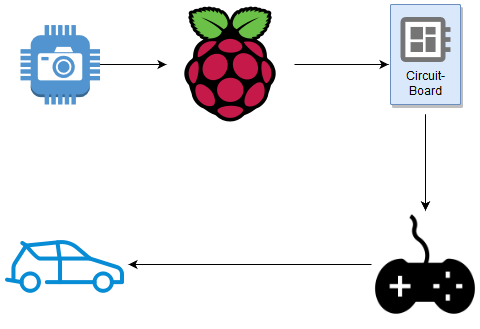
\includegraphics[width=80mm]{SeminarIMMM.png}
        \caption{Архитектура}
        \label{fig:arch}
      \end{figure}
    \end{frame}
    \begin{frame}
      \frametitle{Ограничения}
      \begin{itemize}
        \item{Автомобилът}
          \begin{itemize}
            \item{Постоянна скорост}
            \item{Ограничен ъгъл на завой}
          \end{itemize}
        \item{Камерата}
          \begin{itemize}
            \item{Камерата е фиксирана}
            \item{Ограничен ъгъл на видимост}
            \item{Зависимост от околната среда}
          \end{itemize}
      \end{itemize}
    \end{frame}
\section{Използвани модели и алгоритми}
    \begin{frame}
      \frametitle{Моделиране на движението на колата}
      \begin{itemize}
        \item{\hyperlink{monocycle}{Кинематични модели}}
        \begin{itemize}
          \item{\hyperlink{monocycle}{Едноколесно превозно средство/Unicycle Model/}}
          \item{\hyperlink{bicycle}{Двуколесно превозно средство/Bicycle Model/}}
        \end{itemize}
        \item{\hyperlink{dynamic}{Динамичен модел на двуколесно превозно средство/Dynamic Bicycle Model/}}
      \end{itemize}
    \end{frame}
    \subsection{Кинематични модели}
    \begin{frame}
      \label{monocycle}
      \frametitle{Модел на едноколесно превозно средство\\/Unicycle Model/}
      \only<2>{\framesubtitle{Извеждане на модела}}
      \begin{columns}
      \column{0.5\textwidth}
      \only<1>{\begin{tikzpicture}[scale = 3]}
      \only<2>{\begin{tikzpicture}[scale = 2]
        \clip (-0.5,-0.5) rectangle (3,3);}
        \draw[->, gray] (-0.1,0) -- (1.8,0) coordinate (x axis) node[anchor = north] {$x$};
        \draw[->, gray] (0,-0.1) -- (0,1.8) coordinate (y axis) node[anchor = west] {$y$};
        \draw[rotate = 10,blue] (0.35,0.15) rectangle (1.35, 0.65);
        \draw[rotate = 10, <->] (0.35,0.1) -- (1.35,0.1) node[below =12pt, left = 30pt]{\tiny$l$};
        \filldraw[fill=gray!20,draw=gray!50!black, rotate = 30,thick] (0.95,0.05) circle (0.3cm and 0.12 cm);
        \draw[->, gray] (0.75, 0.5) -- (1.25,0.5);
        \draw[->, gray] (0.75, 0.5) -- (0.75,1);
        \draw[densely dashed, brown, ->] (0.75, 0.5) -- (0.68,1);
        \draw[->] (0.75, 0.5) -- (1.25,0.8);
        \draw[red, thick] (0.95, 0.54) arc (5:18:10pt) node[anchor = west] {\tiny$\beta$};
        \draw[->] (0.75, 0.5) -- (1.35,0.62) node[anchor = north]{\tiny$v$};
        \draw[green, thick] (1.1, 0.5) arc (0:11:10pt) node[anchor = west] {\tiny$\theta$};
        \draw[dashed] (0.75, 0) -- node[below = 20pt]{\tiny x}(0.75, 0.5);
        \draw[dashed] (0, 0.5) -- node[left = 30pt]{\tiny y}(0.75, 0.5);
        \only<2>{
          \draw[densely dashed, green] (1.5, 0.8) node[anchor = west]{\tiny$s$} arc (0:80:100pt);
          \draw[densely dashed,magenta, <->] (0.29, 0.4) node[label={[xshift=-0.5cm, yshift=0.5cm]\tiny R}]{}-- (-0.14,2.7) ;
          \draw[dashed, magenta] (-0.14,2.7) -- (1.27,0.6);
          \draw[densely dashed,magenta] (0.29, 0.4) -- (0.75,0.5);
          } 
      \end{tikzpicture}
      \column{0.5\textwidth}
      \only<1>{\tiny{\begin{block}{Модел}
              \begin{align*}
                \dot{x}      &= v cos(\theta)\\
                \dot{y}      &= v sin(\theta)\\
                \dot{\theta} &= \frac{v tg(\beta)}{l}
              \end{align*}
            \end{block}}
      \tiny{\begin{description}
              \item[$x$]{Позицията по $O_x$}
              \item[$y$]{Позицията по $O_y$}
              \item[$\theta$]{Ъгъла на ориентацията на колата спрямо $O_x$}
              \item[$\beta$]{Ъгъла на завъртане на гумите спрямо ЛКС}
              \item[$l$]{Дължина на оста на автомобила}
            \end{description}}}
      \only<2>{
      \begin{tcolorbox}[colback=red!5!white,colframe=red!75!black]
      \begin{align*}
        \dot{\theta} &= \frac{d\theta}{dt}=\frac{d\theta}{ds}.\frac{ds}{dt}\\
         &= \kappa . v = \frac{1}{R}.v = \frac{tg\beta}{l}.v
      \end{align*}
      \end{tcolorbox}
      }
      \end{columns}
    \end{frame}


    \begin{frame}
      \label{bicycle}
      \frametitle{Модел на двуколесно превозно средство\\/Bicycle Model/}
      \only<2-4>{\framesubtitle{Извеждане на модела}}
      \begin{columns}
      \column{0.5\textwidth}
      
      \begin{tikzpicture}[scale = 1.5]
        \draw[->, gray] (-0.1,0) -- (3.5,0) coordinate (x axis) node[anchor = north] {$x$};
        \draw[->, gray] (0,-0.1) -- (0,3) coordinate (y axis) node[anchor = west] {$y$};
        \filldraw[fill=gray!20,draw=gray!50!black, rotate = 30] (0.95,0.05) circle (0.3cm and 0.12 cm);
        \filldraw[fill=gray!20,draw=gray!50!black, rotate = 80] (1.75,-1.96) circle (0.3cm and 0.12 cm);
        \draw[thick,blue] (0.75, 0.49) -- (2.25,1.35);
        \filldraw[fill=green!20,draw=green!50!black] (1.5,0.94) circle (0.05cm);
        \draw[red, thick] (2.45, 1.48) arc (0:59:10pt) node[anchor = west] {\tiny$\beta$};
        \draw[->] (2.25,1.35) -- (2.35,2.55);
        \draw[->, densely dashed, brown] (2.25, 1.35) -- (3.25, 1.94);
        \draw[->, densely dashed, brown] (2.25, 1.35) -- (1.75, 2.35);
        \draw[->, densely dashed, brown] (1.5,  0.94) -- (1,    1.94);
        \draw[->, densely dashed, brown] (1.5,  0.94) -- (2,  1.2);
        \draw[->, gray] (1.5,0.94) -- (2.5, 0.94);
        \draw[->, gray] (1.5,0.94) -- (1.5, 1.94);
        \draw[green, thick] (1.7, 0.94) arc (0:15:10pt) node[anchor = west]{\tiny{$\theta$}};
        \draw[pink, ->,thick] (1.5,0.94) -- (1.9,1.9) node[anchor = north,red]{\tiny$v$};
        \draw[pink,thick] (1.8, 1.1) arc (0:50:10pt) node[anchor = west,red]{\tiny$\phi$};
        \draw[<->] (1.6,0.7) -- (2.35,1.11) node[left = 10pt, below = 2pt]{\tiny{$l_f$}};
        \draw[<->] (0.85, 0.25) -- (1.6, 0.7) node[left = 10pt, below = 2pt]{\tiny{$l_r$}};
        % \draw[->] (2.25,1.35) -- (3.25,1.15);
        \draw[densely dashed] (1.5,0.94) -- (1.6,0.7);
        \draw[densely dashed] (2.25,1.35) -- (2.35,1.11);
        \draw[densely dashed] (0.75, 0.49) -- (0.85, 0.25);
        \draw[dashed] (1.5, 0) -- node[below = 20pt]{\tiny x}(1.5,0.94);
        \draw[dashed] (0, 0.94) -- node[left = 30pt]{\tiny y}(1.5, 0.94);
        \only<2,3>{
          \draw[gray] (2.25,1.35) node[black, anchor = west]{\tiny B} -- (0.2,1.55) node[black,left = 2pt, anchor = south]{\tiny O};
          \draw[gray] (0.75, 0.49) node[black,anchor = east]{\tiny A} -- (0.2,1.55);
          \draw[gray] (0.75,0.49) -- (1.5,0.94)node[black, anchor = south]{\tiny C};
          \draw[gray] (1.5,0.94) --(0.2,1.55) node[below = 10pt,right = 10pt, black]{\tiny R};
        }
      \end{tikzpicture}
      \column{0.5\textwidth}
      \only<1>{\tiny{\begin{block}{Модел}
              \begin{align*}
                \dot{x}      &= v cos(\theta + \phi)\\
                \dot{y}      &= v sin(\theta + \phi)\\
                \dot{\theta} &= \frac{v}{l_r}sin(\phi)\\
                \phi         &= arctg\left(\frac{l_r}{l_f+l_r}tg(\beta)\right)
              \end{align*}
            \end{block}}
      \tiny{\begin{description}
              \item[$x$]{Позицията на ЦТ по $O_x$}
              \item[$y$]{Позицията на ЦТ по $O_y$}
              \item[$\theta$]{Ъгъла на ориентацията на колата спрямо $O_x$}
              \item[$\beta$]{Ъгъла на завъртане на гумите спямо ЛКС}
              \item[$\phi$]{Ъгъла на скоростта спрямо ориентацията на колата}
              \item[$l_{r/f}$]{Дължина на колата от ЦТ до остта на задните/предните гуми}
            \end{description}}}
        \only<2>{
        \begin{tcolorbox}[colback=red!5!white,colframe=red!75!black]
          \begin{equation*}
          % може директно да се каже понеже е ъглова скорост
            \dot{\theta} = \kappa.v=\frac{1}{R}v=sin(\phi)\frac{v}{l_r} 
          \end{equation*}
        \end{tcolorbox}}
        \only<3>{
        \begin{tcolorbox}[colback=red!5!white,colframe=red!75!black]
        От синусова теорема за $\Delta OCB$
          \begin{align}
          &\frac{sin(\beta-\phi)}{l_f}=\frac{sin\left(\frac{\pi}{2}-\beta\right)}{R}\nonumber\\
          &\Updownarrow\nonumber \\&tan\beta cos\phi-sin\phi = \frac{l_f}{R}
          \end{align}
        и от $\Delta OCA$
          \begin{equation}
            sin\beta = \frac{l_r}{R}
          \end{equation}
        \end{tcolorbox}}
        \only<4>{
        \begin{tcolorbox}[colback=red!5!white,colframe=red!75!black]
          \begin{align*}
            &0=(1).l_r - (2) . l_f =\\&= l_rtg\beta cos\phi - (l_f+l_r)sin\phi\\
            &tg\phi = \frac{l_rtg\beta}{l_f+l_r}\\
            &\Leftrightarrow\phi=arctg\frac{l_rtg\beta}{l_f+l_r}
          \end{align*}
        \end{tcolorbox}
        }
      \end{columns}
      % начертай си вкъщи триъгълниците и нещата и виж там некви синусови и тригонометрия и вафли
      % youtube and coursera may be 
    \end{frame}
    \subsection{Динамичен модел}
    \label{dynamic}
    \subsection{Динамичен модел}
    \label{dynamic}
    \begin{frame}
      \frametitle{Динамичен модел на двуколесно превозно средство\\/Dynamic Bicycle Model/}
      \begin{columns}
      \column{0.5\textwidth}
      
      
      \begin{tikzpicture}[scale = 1.5]
        \draw[->, gray] (-0.1,0) -- (3.8,0) coordinate (x axis) node[anchor = north] {$x$};
        \draw[->, gray] (0,-0.1) -- (0,3) coordinate (y axis) node[anchor = west] {$y$};
        \filldraw[fill=gray!20,draw=gray!50!black, rotate = 30] (0.95,0.05) circle (0.3cm and 0.12 cm);
        \filldraw[fill=gray!20,draw=gray!50!black, rotate = 80] (1.75,-1.96) circle (0.3cm and 0.12 cm);
        \draw[thick,blue] (0.75, 0.49) -- (2.25,1.35);
        \filldraw[fill=green!20,draw=green!50!black] (1.5,0.94) circle (0.05cm);
        \draw[red, thick] (2.45, 1.48) arc (0:59:10pt) node[anchor = west] {\tiny$\beta$};
        \draw[->] (2.25,1.35) -- (2.35,2.55);
        \draw[->, densely dashed, brown] (2.25, 1.35) -- (3.25, 1.94);
        \draw[->, densely dashed, brown] (2.25, 1.35) -- (1.75, 2.35);
        \draw[->, densely dashed, brown] (1.5,  0.94) -- (1,    1.94)node[anchor=north]{\tiny$y$};
        \draw[->, densely dashed, brown] (1.5,  0.94) -- (2,  1.2)node[anchor=north]{\tiny$x$};
        \draw[->, gray] (1.5,0.94) -- (2.5, 0.94);
        \draw[->, gray] (1.5,0.94) -- (1.5, 1.94);
        \draw[green, thick] (1.7, 0.94) arc (0:15:10pt) node[anchor = west]{\tiny{$\theta$}};
        \draw[pink, ->,thick] (1.5,0.94) -- (1.75,0.5) node[anchor = north,red]{\tiny$v$};
theta     \draw[<->] (1.6,0.7) -- (2.35,1.11) node[left = 15pt, below = 4pt]{\tiny{$l_f$}};
        \draw[<->] (0.85, 0.25) -- (1.6, 0.7) node[left = 10pt, below = 2pt]{\tiny{$l_r$}};
        \draw[densely dashed] (1.5,0.94) -- (1.6,0.7);
        \draw[densely dashed] (2.25,1.35) -- (2.35,1.11);
        \draw[densely dashed] (0.75, 0.49) -- (0.85, 0.25);
        \draw[dashed] (1.5, 0) -- node[below = 20pt]{\tiny $X$}(1.5,0.94);
        \draw[dashed] (0, 0.94) -- node[left = 30pt]{\tiny $Y$}(1.5, 0.94);
        \draw[->, thick] (2.25,1.35) -- (2.8,1.3) node[right=1pt]{\tiny$F_{c,f}$};
        \draw[->, thick] (0.75, 0.49) -- (1, 0.05) node [left=1pt]{\tiny$F_{c,r}$};
      \end{tikzpicture}
      \column{0.5\textwidth}
      \only<1>{\tiny{\begin{block}{Модел}
              \begin{align*}
                \ddot{x}      &= \dot{\theta}\dot{y}\\
                \ddot{y}      &= -\dot{\theta}\dot{x} + \frac{2}{m}(F_{c,f}cos\beta + F_{c,r})\\
                \ddot{\theta}   &= \frac{2}{I_z}(l_f F_{c,f} - l_r F_{c,r}))\\
                \dot{X}       &= \dot{x}cos\theta-\dot{y}sin\theta\\
                \dot{Y}       &= \dot{x}sin\theta+\dot{y}cos\theta
              \end{align*}
            \end{block}}
      \tiny{\begin{description}
              \item[$X$]{Позицията на ЦТ по $O_x$}
              \item[$Y$]{Позицията на ЦТ по $O_y$}
              \item[$\theta$]{Ъгъла на ориентацията на колата}
              \item[$\beta$]{Ъгъла на завъртане на гумите}
              \item[$l_{r/f}$]{Дължина на колата от ЦТ до остта на задните/предните гуми}
              \item[$F_{c,r/f}$]{Силите при задните/предните гуми}
              \item[$I_z$]{инерциална маса}
            \end{description}}}
        \only<2>{
          $F_{c,r/f}$ са базирани на линейния модел на гумите
          \begin{tcolorbox}[colback=red!5!white,colframe=red!75!black]
          $F_{c,f/r}=-C_{\alpha_{r/f}\alpha_{r/f}}$
          \end{tcolorbox}
          Където 
          $\alpha_{r/f}$ е ъгъла на приплъзване съответно за задната/предната гума и $C_{\alpha_{r/f}}$ е коефициент за сцеплението при завой.
        }
      \end{columns}
    \end{frame}
    % \begin{frame}
    %   \frametitle{Реализация}
    %   \begin{itemize}
    %     \item{Кинематичния модел на двуколесно ПС - $l_f=l_r=l/2$}
    %     \item{Динамичния модел на двуколесно ПС - $F_{c,r/f}$ се базират на линейния модел на гумите}
    %     \begin{itemize}
    %       \item{$F_{c,f/r}=-C_{\alpha_{r/f}\alpha_{r/f}}$,където 
    %       $\alpha_{r/f}$ е ъгъла на приплъзване съответно за задната/предната гума и $C_{\alpha_{r/f}}$ е коефициент за сцеплението при завой.}

    %     \end{itemize}
    %   \end{itemize}
    % \end{frame}
    \subsection{Намиране на маршрут}
    \begin{frame}
      \frametitle{Намиране на маршрут}
      \framesubtitle{Търсене Hybrid A*}
      Проблем:
         \begin{itemize}
          \item{Дискретни алгоритми за търсене}
          \item{Непрекъснато пространство от състояния на автомобила}
          \item{Твърде широко дърво за търсене}
          \item{Избиране на подходяща евристика}
        \end{itemize}
    \end{frame}
    \begin{frame}
      \frametitle{Разлика между Дийкстра, А*}
      \only<1>{
      \begin{figure}
        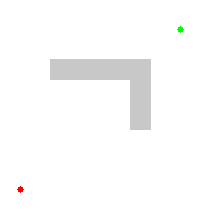
\includegraphics[width=60mm]{Search_Start.png}
        \caption{Начално състоние}
        \label{fig:search}
      \end{figure}
      }
      \only<2>{
      \begin{columns}
        \column{0.5\textwidth}
        \begin{figure}
        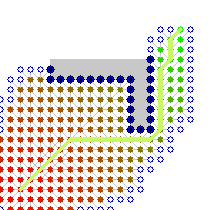
\includegraphics[width=40mm]{Astar_End.png}
        \caption{Крайно състояние, А*}
        \label{fig:astar}
      \end{figure}
        % \movie[autostart, loop, showcontrols]{}{Dijkstras_progress_animation.avi}
        \column{0.5\textwidth}
        \begin{figure}
        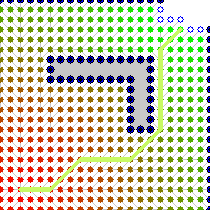
\includegraphics[width=40mm]{Dijkstra_End.png}
        \caption{Крайно състояние, Дийкстра}
        \label{fig:dij}
      \end{figure}
        % слага цена само на центъра на състоянието
        % \movie[autostart, loop, showcontrols]{}{Dijkstras_progress_animation.avi}
      \end{columns}}
    \end{frame}
    \begin{frame}
      \frametitle{Защо хибриден?}
      \begin{columns}
      \column{0.5\textwidth}
      \begin{center}
        \begin{tikzpicture}[scale=3]
          \draw[step=.5cm,gray,very thin] (-0.5,-0.5) grid (1,1);
          \draw[->,green] (0.25,0.25) -- (0.25,0.75);
          \draw[densely dashed, gray] (0.25,0.75) circle (0.1);
          \draw[->,green] (0.25,0.25) .. controls +(30:0.5cm) .. (0.75,0.75);
          \draw[densely dashed, gray] (0.75,0.75) circle (0.1);
          \draw[->,green] (0.25,0.25) .. controls +(150:0.5cm) .. (-0.25,0.75);
          \draw[densely dashed, gray] (-0.25,0.75) circle (0.1);
          \draw[->,green] (0.25,0.25) .. controls +(65:0.5cm) .. (0.45,0.75);
          \draw[densely dashed, gray] (0.45,0.75) circle (0.1);
          \draw[->,green] (0.25,0.25) .. controls +(120:0.5cm) .. (0.05,0.75);
          \draw[densely dashed, gray] (0.05,0.75) circle (0.1);
          \draw[->,red] (0.25,0.25) --(-0.25,0.25); 
          \draw (-0.3,0.25) node[cross,thick,scale = 3,red]{};
          \draw[->,red] (0.2,0.25) -- (0.75,0.25);
          \draw (0.8,0.25) node[cross,thick,scale = 3, red]{};
          \draw[->,blue] (0.25,0.25) -- (0.25,-0.25);
          \draw[densely dashed, gray] (0.25,-0.25) circle (0.1) node[anchor = north, blue]{\tiny ?};
          \draw[->,blue] (0.25,0.25) .. controls +(330:0.5cm) .. (0.75,-0.25);
          \draw[densely dashed, gray] (0.75,-0.25) circle (0.1) node[anchor = north, blue]{\tiny ?};
          \draw[->,blue] (0.25,0.25) .. controls +(210:0.5cm) .. (-0.25,-0.25);
          \draw[densely dashed, gray] (-0.25,-0.25) circle (0.1) node[anchor = north, blue]{\tiny ?};
          \filldraw[black] (0.25,0.25) circle (0.1);
          \draw[->, green](-0.5,-0.7) -- (-0.4,-0.7) node[right = 10pt]{\tiny Позволено};
          \draw[->,blue] (0.3,-0.7) -- (0.4,-0.7) node[right = 10pt]{\tinyСамо на заден ход};
          \draw[->,red] (0,-0.9) -- (0.1,-0.9) node[right = 10pt]{\tinyНевъзможно};
        \end{tikzpicture}
      \end{center}
      \column{0.5\textwidth}
      \tiny\begin{alertblock}{\tinyФормула за дискретизиране}
        \begin{equation*}
          \widetilde{x} = \frac{x-o_m}{\xi}
        \end{equation*}
      \end{alertblock}
      \begin{flushleft}
      \tiny\begin{description}
          \item[$\widetilde{x}$]{Дискретни координати}
          \item[$o_m$]{Начало на КС}
          \item[$\xi$]{Дължина на клетката}
        \end{description}
      \end{flushleft}
      \tiny\begin{alertblock}{\tinyПредставяне на състоянието}
        \begin{equation*}
          n = \left(\widetilde{x},\theta,x,g,f,n_p\right)
        \end{equation*}
      \end{alertblock}
      \begin{description}
        \item[$x$]{Позиция на колата в КС}
        \item[$g$]{Реална цена за стигане до това състояние}
        \item[$f$]{Сума на реалната цена ($g$) и евристичната за стигане до целта($h$)}
        \item[$n_p$]{Предходно състояние}
      \end{description}
      \end{columns}
    \end{frame}
    \begin{frame}
    % тук с каринка е по-добре ама ме мързи
      \frametitle{Hybrid A*}
      \begin{algorithm}[H]
        \caption{Hybrid A*}\label{has}
        \begin{algorithmic}[1]
          \Procedure{planPath}{$m, \mu, x_s, \theta_sm G$}
            \State{$n_s \leftarrow (\widetilde{x_s},\widetilde{\theta_s},x_s,0,h(x_s,G),-)$}
            \State{$O \leftarrow \{n_s\}$}
            \State {$C\leftarrow \emptyset$}
            \While{$O \neq \emptyset$}
              \State{$n\leftarrow$ node with min $f$ value in $O$}
              \State{$O\leftarrow O\setminus\{n\}$}
              \State{$C\leftarrow C\cup \{n\}$}
              \If{$n_x\in G$}
                \State{\textbf{return} reconstructed path}
              \Else{
                updateNeighbours($m,\mu,O,C,n$)}
              \EndIf
            \EndWhile
            \State{\textbf{return} no path found}
          \EndProcedure
        \end{algorithmic}
      \end{algorithm}
    \end{frame}
    \subsection*{Намиране на местоположението камерата спрямо равнината на движение}
    \begin{frame}
      \frametitle{Намиране на местоположението камерата спрямо равнината на движение}
      \framesubtitle{Калибровка посредством използване на шахматен шаблон}
      \begin{columns}
      \column{0.5\textwidth}
      \begin{itemize}
        \item{Регистриране на ъглите на квадратчетата}
        \item{Намиране на хомографска трансформация между координатите в изображението и идеален модел на шаблона.}
      \end{itemize}
      \column{0.5\textwidth}
      \begin{figure}
        
\includegraphics[width=40mm]{chessboard.jpg}
        \caption{Шахматен шаблон}
        \label{fig:chess}
      \end{figure}
      \end{columns}
    \end{frame}

    % https://pdfs.semanticscholar.org/6e00/16024b257040db590d2de352556f64f46787.pdf

    \subsection*{Намиране на местоположението автомобила}
    \begin{frame}
      \frametitle{Намиране на местоположението автомобила}
      \framesubtitle{Проследяване на фийчъри}
      \begin{columns}
      \column{0.4\textwidth}
      \begin{itemize}
        \item{Регистриране на фийчърите в изображението чрез ORB дескриптор}
        \item{Намиране на фийчърите на автомобила чрез сравнение с предварително известните му фийчъри.}
      \end{itemize}
      \column{0.6\textwidth}
      \begin{figure}
        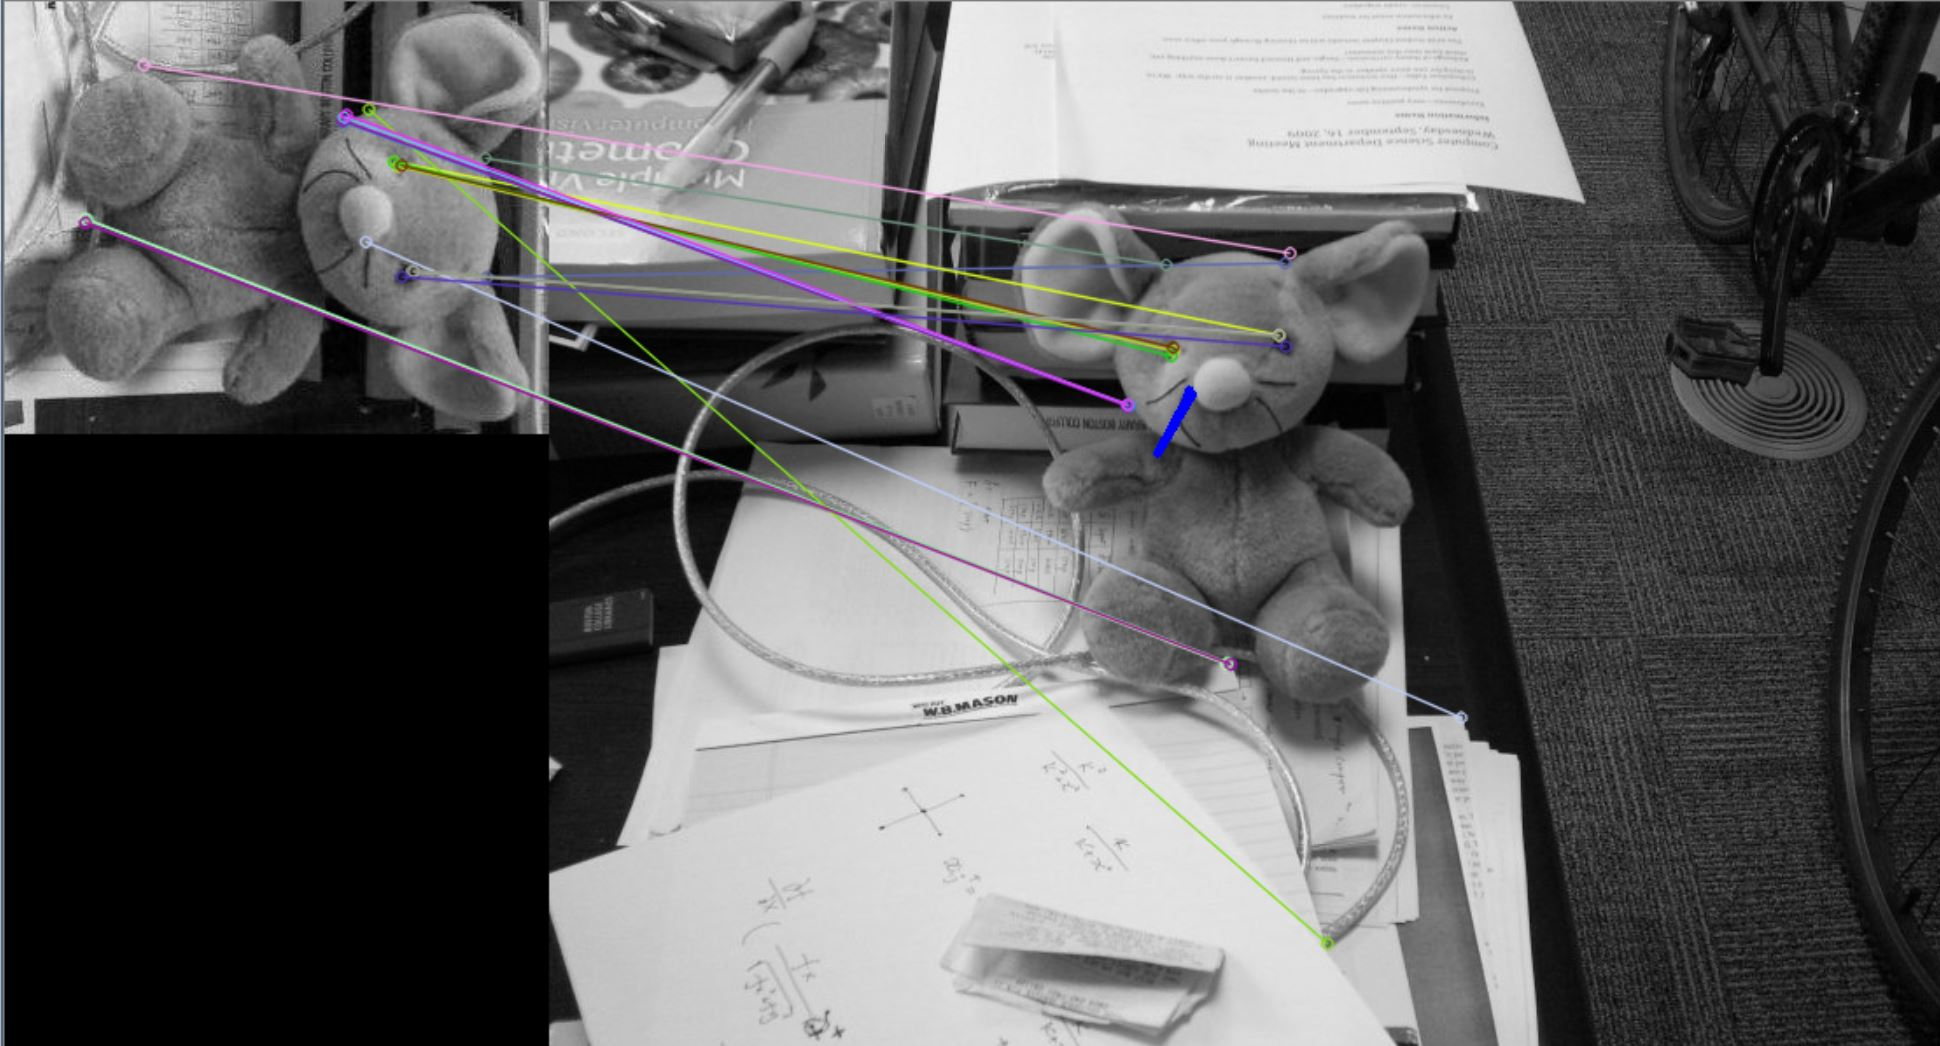
\includegraphics[width=70mm]{ORBpicture.jpg}
        \caption{ORB}
        \label{fig:orb}
      \end{figure}
      \end{columns}
    \end{frame}
  % \section{Демо}
  %   \begin{frame}[plain]
  %     % клипче на колата в движение???
  %     % клипче на демото н алгоритмите
  %     % или самото демо
  %     % пускане на фийчър тракинга
  %     \begin{center}
  %     \Huge{ДЕМО}
  %     \end{center}
  %   \end{frame}
  \section{Обобщение}
    \begin{frame}
      \frametitle{Обобщение}
        \begin{itemize}
          \item{Използват се главно прости модели с до две колела и се коригират грешките със сензори}
          \item{За намиране на траектория не могат да се използват стандартните дискретни алгоритми}
          \item{Подхода за проследяване използван в момента е приложим само за частни случаи}
        \end{itemize}

    \end{frame}
  \section{Бъдеща работа}
  % http://ai.stanford.edu/~ddolgov/papers/dolgov_gpp_stair08.pdf
    \begin{frame}
    \frametitle{Бъдеща работа}
     \begin{itemize}
      \item{Използване на информация от сензори}
      \item{Добавяне на алгоритми за заглаждане на траекторията}
      \item{Добавяне на други евристики при търсенето}
      \item{Имплементиране на динамичния модел и използването му за сравнение}
      \item{Имплементиране на по устойчив към промени в околната среда метод за проследяване}
    \end{itemize}  
    \end{frame}
  \section{Използвана литература}
    \begin{frame}
      \frametitle{Използвана литература}
      \begin{itemize}
        \item[]{\hyperlink{https://pdfs.semanticscholar.org/6e00/16024b257040db590d2de352556f64f46787.pdf}{Petereit, J., Emter, T., Frey, C., Kopfstedt, T., Beutel, A., 2012, Application of Hybrid A* to an Autonomous Mobile Robot forPath Planning in Unstructured Outdoor Environments, ROBOTIK}}
        \item[]{\hyperlink{https://borrelli.me.berkeley.edu/pdfpub/IV_KinematicMPC_jason.pdf}{Kong, J., Pfeiffer, M., Schildbach, G., Borrell, F., 2015, Kinematic  and  Dynamic  Vehicle  Models  for  Autonomous  DrivingControl  Design, IEEE}}
        \item[]{\hyperlink{http://www.robesafe.com/personal/sotelo/RASLateralControl2003.pdf}{Sotelo, M.,2003, Lateral control strategy for autonomous steeringof Ackerman-like vehicles, RAS}}
      \end{itemize}
     \end{frame}
% etc
\end{document}